% Cover
\imprimircapa

% False cover sheet
%\imprimirfalsafolhaderosto

% Cover sheet
\imprimirfolhaderosto

% Card Catalog
\begin{fichacatalografica}
	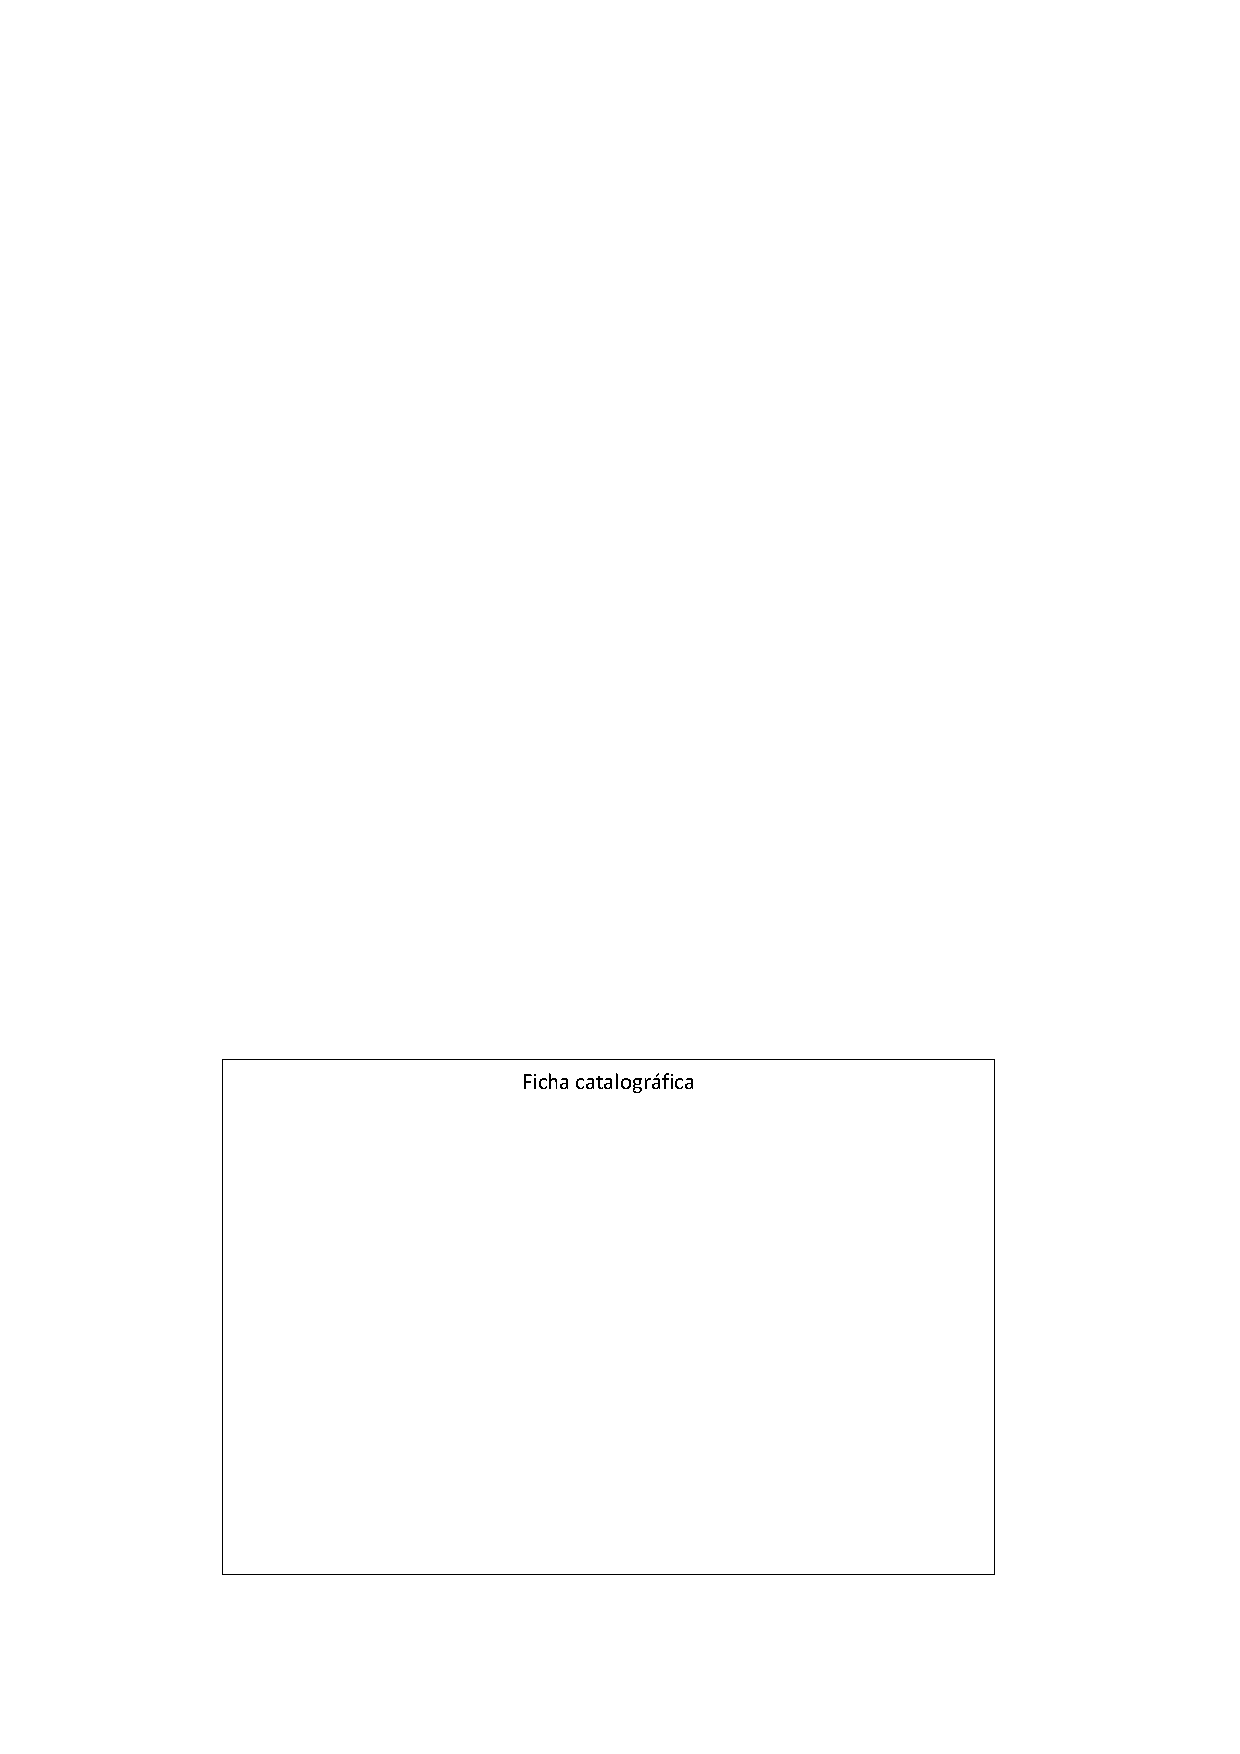
\includepdf{card-catalog.pdf}
\end{fichacatalografica}

% Approval sheet
%\begin{folhadeaprovacao}
%	
%	\begin{center}
%		{\ABNTEXchapterfont\large\imprimirautor}
%		
%		\vspace*{\fill}\vspace*{\fill}
%		\begin{center}
%			\ABNTEXchapterfont\bfseries\Large\imprimirtitulo
%		\end{center}
%		\vspace*{\fill}
%		
%		\hspace{.45\textwidth}
%		\begin{minipage}{.5\textwidth}
%			\imprimirpreambulo
%		\end{minipage}%
%		\vspace*{\fill}
%	\end{center}
%	
%	%Trabalho aprovado. \imprimirlocal, 31 de dezembro de 2020:
%	
%	\assinatura{\textbf{\imprimirorientador} \\ Orientador} 
%	\assinatura{\textbf{\imprimircoorientador} \\ Coorientador} 
%	\assinatura{\textbf{A} \\ Convidado 1}
%	\assinatura{\textbf{B} \\ Convidado 2}
%	
%	\begin{center}
%		\vspace*{0.5cm}
%		{\large\imprimirlocal}
%		\par
%		{\large\imprimirdata}
%		\vspace*{1cm}
%	\end{center}
%	
%\end{folhadeaprovacao}

% Abstract - Portuguese
\setlength{\absparsep}{18pt} % Spacing
\begin{resumo}
	A mudança de paradigma na indústria referente às recentes modificações em relação às tecnologias de manufatura é chamada de Indústria 4.0 (I4.0). Neste novo conceito, redes inteligentes de máquinas e processos para indústria com o respaldo das Tecnologias da Informação e Comunicação (TIC) passam a proporcionar um alto nível de automação e intercâmbio de informações entre equipamentos, produtos e demais atores em um ambiente de manufatura. Este trabalho aborda o aspecto de intercâmbio de informações, mais especificamente o compartilhamento da memória digital do produto (MDP) ao longo da cadeia de suprimentos (CS). Para tal fim, é elaborada uma arquitetura baseada no Modelo de Arquitetura de Referência para a Indústria 4.0 (RAMI4.0). Nesta arquitetura, a MDP é compartilhada por meio de \textit{Web Services} e é composta por três componentes básicos: o servidor de informações (o produto), o cliente consumidor de informações (cada elo da CS) e o repositório, que contém as descrições dos serviços ofertados pelo servidor. Além disso, este trabalho faz o levantamento dos tipos de informações sobre o produto a serem compartilhados ao longo da CS e o impacto em geração de valor que este compartilhamento durante o ciclo do produto traz sobre o negócio.

	\vspace{\onelineskip}

	\noindent
	\textbf{Palavras-chave}: Indústria 4.0. RAMI4.0. Memória digital do produto. Arquitetura orientada a serviços. Cadeia de suprimentos.
\end{resumo}

% Abstract - English
\begin{resumo}[Abstract]
	\begin{otherlanguage*}{english}
		The paradigm shift in the industry regarding the recent changes in manufacturing technologies is called Industry 4.0 (I4.0). In this new concept, intelligent networks of machines and processes for industry with the support of Information and Communication Technologies (ICT) start to provide a high level of automation and exchange of information between equipment, products and other actors in a manufacturing environment. This work addresses the information exchange aspect, more specifically the sharing of the Digital Product Memory (DPM) along the supply chain (SC). To this end, an architecture based on the Reference Architectural Model Industrie 4.0 (RAMI4.0) is developed. In this architecture, the DPM is shared through \textit{Web Services} and it's composed of three basic components: the server of information (the product), the client consuming that information (each link of the SC) and the repository, which contains descriptions of the services offered by the server. In addition, this work surveys the types of information about the product to be shared along the SC and the impact on value generation that this sharing during the product cycle has on the business.

		\vspace{\onelineskip}

		\noindent
		\textbf{Keywords}: Industry 4.0. RAMI4.0. Digital product memory. Service-oriented architecture. Supply chain.
	\end{otherlanguage*}
\end{resumo}

% List of illustrations
\pdfbookmark[0]{\listfigurename}{lof}
\listoffigures*
\cleardoublepage

% List of tables
\pdfbookmark[0]{\listtablename}{lot}
\listoftables*
\cleardoublepage

% List of abbreviations and acronyms
\begin{siglas}
	\item[AAS] \textit{Asset Administration Shell} (Casca Administrativa do Ativo)
	\item[API] \textit{Application Programming Interface} (Interface de Programação de Aplicação)
	\item[BD] Banco de Dados
	\item[BI] \textit{Business Intelligence} (Inteligência Empresarial)
	\item[BOM] \textit{Bill of Materials} (Lista de Materiais)
	\item[C4.0] Componente 4.0
	\item[CRUD] \textit{Create, Read, Update, Delete} (Criação, Leitura, Atualização, Exclusão)
	\item[CS] Cadeia de Suprimentos
	\item[CV] Cadeia de Valor
	\item[CVP] Ciclo de Vida do Produto
	\item[GCVP] Gestão do Ciclo de Vida do Produto
	\item[GI] Gestão da Informação
	\item[I4.0] Indústria 4.0
	\item[IIoT] \textit{Industrial Internet of Things} (Internet das Coisas Industrial)
	\item[IoT] \textit{Internet of Things} (Internet das Coisas)
	\item[JSON] \textit{JavaScript Object Notation} (Notação de Objeto do JavaScript)
	\item[LGPD] Lei Geral de Proteção de Dados
	\item[MDP] Memória Digital do Produto
	\item[OEE] \textit{Overall Equipment Effectiveness} (Eficiência Global do Equipamento)
	\item[OSI] \textit{Open System Interconnection} (Interconexão Aberta de Sistemas)
	\item[PFS] \textit{Production Flow Schema} (Esquema de Fluxo de Produção)
	\item[QoS] \textit{Quality of Service} (Qualidade de Serviço)
	\item[RAMI4.0] \textit{Reference Architectural Model Industrie 4.0} (Modelo de Arquitetura de Referência para a Indústria 4.0)
	\item[REST] \textit{Representational State Transfer} (Transferência Representacional de Estado)
	\item[RFID] (\textit{Radio-Frequency IDentification}) (Identificação por Radiofrequência)
	\item[SOA] \textit{Service Oriented Architecture} (Arquitetura Orientada a Serviços)
	\item[SOAP] \textit{Simple Object Access Protocol} (Protocolo para Simples Acesso de Objetos)
	\item[SED] Sistemas a eventos discretos
	\item[TIC] Tecnologia da Informação e Comunicação
	\item[UUID] \textit{Universal Unique IDentifier} (Identificador Único Universal)
	\item[WS] \textit{Web Service} (Serviço Web)
	\item[WSD] \textit{Web Services Description} (Descrição do Serviço Web)
	\item[WSDL] \textit{Web Services Description Language} (Linguagem de Descrição de Serviços Web)
	\item[XML] \textit{Extensible Markup Language} (Linguagem Extensível de Marcação)
\end{siglas}

% Summary
\pdfbookmark[0]{\contentsname}{toc}
\tableofcontents*
\cleardoublepage
